% Options for packages loaded elsewhere
\PassOptionsToPackage{unicode}{hyperref}
\PassOptionsToPackage{hyphens}{url}
%
\documentclass[
  12pt,
]{article}
\usepackage{amsmath,amssymb}
\usepackage{iftex}
\ifPDFTeX
  \usepackage[T1]{fontenc}
  \usepackage[utf8]{inputenc}
  \usepackage{textcomp} % provide euro and other symbols
\else % if luatex or xetex
  \usepackage{unicode-math} % this also loads fontspec
  \defaultfontfeatures{Scale=MatchLowercase}
  \defaultfontfeatures[\rmfamily]{Ligatures=TeX,Scale=1}
\fi
\usepackage{lmodern}
\ifPDFTeX\else
  % xetex/luatex font selection
    \setmainfont[]{Times New Roman}
\fi
% Use upquote if available, for straight quotes in verbatim environments
\IfFileExists{upquote.sty}{\usepackage{upquote}}{}
\IfFileExists{microtype.sty}{% use microtype if available
  \usepackage[]{microtype}
  \UseMicrotypeSet[protrusion]{basicmath} % disable protrusion for tt fonts
}{}
\makeatletter
\@ifundefined{KOMAClassName}{% if non-KOMA class
  \IfFileExists{parskip.sty}{%
    \usepackage{parskip}
  }{% else
    \setlength{\parindent}{0pt}
    \setlength{\parskip}{6pt plus 2pt minus 1pt}}
}{% if KOMA class
  \KOMAoptions{parskip=half}}
\makeatother
\usepackage{xcolor}
\usepackage[margin=1in]{geometry}
\usepackage{color}
\usepackage{fancyvrb}
\newcommand{\VerbBar}{|}
\newcommand{\VERB}{\Verb[commandchars=\\\{\}]}
\DefineVerbatimEnvironment{Highlighting}{Verbatim}{commandchars=\\\{\}}
% Add ',fontsize=\small' for more characters per line
\usepackage{framed}
\definecolor{shadecolor}{RGB}{248,248,248}
\newenvironment{Shaded}{\begin{snugshade}}{\end{snugshade}}
\newcommand{\AlertTok}[1]{\textcolor[rgb]{0.94,0.16,0.16}{#1}}
\newcommand{\AnnotationTok}[1]{\textcolor[rgb]{0.56,0.35,0.01}{\textbf{\textit{#1}}}}
\newcommand{\AttributeTok}[1]{\textcolor[rgb]{0.13,0.29,0.53}{#1}}
\newcommand{\BaseNTok}[1]{\textcolor[rgb]{0.00,0.00,0.81}{#1}}
\newcommand{\BuiltInTok}[1]{#1}
\newcommand{\CharTok}[1]{\textcolor[rgb]{0.31,0.60,0.02}{#1}}
\newcommand{\CommentTok}[1]{\textcolor[rgb]{0.56,0.35,0.01}{\textit{#1}}}
\newcommand{\CommentVarTok}[1]{\textcolor[rgb]{0.56,0.35,0.01}{\textbf{\textit{#1}}}}
\newcommand{\ConstantTok}[1]{\textcolor[rgb]{0.56,0.35,0.01}{#1}}
\newcommand{\ControlFlowTok}[1]{\textcolor[rgb]{0.13,0.29,0.53}{\textbf{#1}}}
\newcommand{\DataTypeTok}[1]{\textcolor[rgb]{0.13,0.29,0.53}{#1}}
\newcommand{\DecValTok}[1]{\textcolor[rgb]{0.00,0.00,0.81}{#1}}
\newcommand{\DocumentationTok}[1]{\textcolor[rgb]{0.56,0.35,0.01}{\textbf{\textit{#1}}}}
\newcommand{\ErrorTok}[1]{\textcolor[rgb]{0.64,0.00,0.00}{\textbf{#1}}}
\newcommand{\ExtensionTok}[1]{#1}
\newcommand{\FloatTok}[1]{\textcolor[rgb]{0.00,0.00,0.81}{#1}}
\newcommand{\FunctionTok}[1]{\textcolor[rgb]{0.13,0.29,0.53}{\textbf{#1}}}
\newcommand{\ImportTok}[1]{#1}
\newcommand{\InformationTok}[1]{\textcolor[rgb]{0.56,0.35,0.01}{\textbf{\textit{#1}}}}
\newcommand{\KeywordTok}[1]{\textcolor[rgb]{0.13,0.29,0.53}{\textbf{#1}}}
\newcommand{\NormalTok}[1]{#1}
\newcommand{\OperatorTok}[1]{\textcolor[rgb]{0.81,0.36,0.00}{\textbf{#1}}}
\newcommand{\OtherTok}[1]{\textcolor[rgb]{0.56,0.35,0.01}{#1}}
\newcommand{\PreprocessorTok}[1]{\textcolor[rgb]{0.56,0.35,0.01}{\textit{#1}}}
\newcommand{\RegionMarkerTok}[1]{#1}
\newcommand{\SpecialCharTok}[1]{\textcolor[rgb]{0.81,0.36,0.00}{\textbf{#1}}}
\newcommand{\SpecialStringTok}[1]{\textcolor[rgb]{0.31,0.60,0.02}{#1}}
\newcommand{\StringTok}[1]{\textcolor[rgb]{0.31,0.60,0.02}{#1}}
\newcommand{\VariableTok}[1]{\textcolor[rgb]{0.00,0.00,0.00}{#1}}
\newcommand{\VerbatimStringTok}[1]{\textcolor[rgb]{0.31,0.60,0.02}{#1}}
\newcommand{\WarningTok}[1]{\textcolor[rgb]{0.56,0.35,0.01}{\textbf{\textit{#1}}}}
\usepackage{longtable,booktabs,array}
\usepackage{calc} % for calculating minipage widths
% Correct order of tables after \paragraph or \subparagraph
\usepackage{etoolbox}
\makeatletter
\patchcmd\longtable{\par}{\if@noskipsec\mbox{}\fi\par}{}{}
\makeatother
% Allow footnotes in longtable head/foot
\IfFileExists{footnotehyper.sty}{\usepackage{footnotehyper}}{\usepackage{footnote}}
\makesavenoteenv{longtable}
\usepackage{graphicx}
\makeatletter
\def\maxwidth{\ifdim\Gin@nat@width>\linewidth\linewidth\else\Gin@nat@width\fi}
\def\maxheight{\ifdim\Gin@nat@height>\textheight\textheight\else\Gin@nat@height\fi}
\makeatother
% Scale images if necessary, so that they will not overflow the page
% margins by default, and it is still possible to overwrite the defaults
% using explicit options in \includegraphics[width, height, ...]{}
\setkeys{Gin}{width=\maxwidth,height=\maxheight,keepaspectratio}
% Set default figure placement to htbp
\makeatletter
\def\fps@figure{htbp}
\makeatother
\setlength{\emergencystretch}{3em} % prevent overfull lines
\providecommand{\tightlist}{%
  \setlength{\itemsep}{0pt}\setlength{\parskip}{0pt}}
\setcounter{secnumdepth}{5}
% definitions for citeproc citations
\NewDocumentCommand\citeproctext{}{}
\NewDocumentCommand\citeproc{mm}{%
  \begingroup\def\citeproctext{#2}\cite{#1}\endgroup}
\makeatletter
 % allow citations to break across lines
 \let\@cite@ofmt\@firstofone
 % avoid brackets around text for \cite:
 \def\@biblabel#1{}
 \def\@cite#1#2{{#1\if@tempswa , #2\fi}}
\makeatother
\newlength{\cslhangindent}
\setlength{\cslhangindent}{1.5em}
\newlength{\csllabelwidth}
\setlength{\csllabelwidth}{3em}
\newenvironment{CSLReferences}[2] % #1 hanging-indent, #2 entry-spacing
 {\begin{list}{}{%
  \setlength{\itemindent}{0pt}
  \setlength{\leftmargin}{0pt}
  \setlength{\parsep}{0pt}
  % turn on hanging indent if param 1 is 1
  \ifodd #1
   \setlength{\leftmargin}{\cslhangindent}
   \setlength{\itemindent}{-1\cslhangindent}
  \fi
  % set entry spacing
  \setlength{\itemsep}{#2\baselineskip}}}
 {\end{list}}
\usepackage{calc}
\newcommand{\CSLBlock}[1]{\hfill\break\parbox[t]{\linewidth}{\strut\ignorespaces#1\strut}}
\newcommand{\CSLLeftMargin}[1]{\parbox[t]{\csllabelwidth}{\strut#1\strut}}
\newcommand{\CSLRightInline}[1]{\parbox[t]{\linewidth - \csllabelwidth}{\strut#1\strut}}
\newcommand{\CSLIndent}[1]{\hspace{\cslhangindent}#1}
\usepackage{tcolorbox}
\usepackage{amssymb}
\usepackage{yfonts}
\usepackage{bm}
\usepackage{titlesec}
\usepackage{kbordermatrix}


\newtcolorbox{greybox}{
  colback=white,
  colframe=blue,
  coltext=black,
  boxsep=5pt,
  arc=4pt}
  
\newcommand{\sectionbreak}{\clearpage}

 
\newcommand{\ds}[4]{\sum_{{#1}=1}^{#3}\sum_{{#2}=1}^{#4}}
\newcommand{\us}[3]{\mathop{\sum\sum}_{1\leq{#2}<{#1}\leq{#3}}}

\newcommand{\ol}[1]{\overline{#1}}
\newcommand{\ul}[1]{\underline{#1}}

\newcommand{\amin}[1]{\mathop{\text{argmin}}_{#1}}
\newcommand{\amax}[1]{\mathop{\text{argmax}}_{#1}}

\newcommand{\ci}{\perp\!\!\!\perp}

\newcommand{\mc}[1]{\mathcal{#1}}
\newcommand{\mb}[1]{\mathbb{#1}}
\newcommand{\mf}[1]{\mathfrak{#1}}

\newcommand{\eps}{\epsilon}
\newcommand{\lbd}{\lambda}
\newcommand{\alp}{\alpha}
\newcommand{\df}{=:}
\newcommand{\am}[1]{\mathop{\text{argmin}}_{#1}}
\newcommand{\ls}[2]{\mathop{\sum\sum}_{#1}^{#2}}
\newcommand{\ijs}{\mathop{\sum\sum}_{1\leq i<j\leq n}}
\newcommand{\jis}{\mathop{\sum\sum}_{1\leq j<i\leq n}}
\newcommand{\sij}{\sum_{i=1}^n\sum_{j=1}^n}
	
\ifLuaTeX
  \usepackage{selnolig}  % disable illegal ligatures
\fi
\usepackage{bookmark}
\IfFileExists{xurl.sty}{\usepackage{xurl}}{} % add URL line breaks if available
\urlstyle{same}
\hypersetup{
  pdfauthor={Jan de Leeuw - University of California Los Angeles},
  hidelinks,
  pdfcreator={LaTeX via pandoc}}

\title{Smacof at 50: A Manual\\
Part 1: Smacof with B-Splines}
\author{Jan de Leeuw - University of California Los Angeles}
\date{Started February 21 2024, Version of April 16, 2024}

\begin{document}
\maketitle
\begin{abstract}
TBD
\end{abstract}

{
\setcounter{tocdepth}{4}
\tableofcontents
}
\textbf{Note:} This is a working manuscript which will be expanded/updated
frequently. All suggestions for improvement are welcome. All Rmd, tex,
html, pdf, R, and C files are in the public domain. Attribution will be
appreciated, but is not required. The files can be found at
\url{https://github.com/deleeuw/smacofCode}.

\sectionbreak

\section{Smacof Algorithm}\label{smacof-algorithm}

\subsection{First Phase: Update Configuration}\label{first-phase-update-configuration}

\subsubsection{Introduction to Majorization}\label{introduction-to-majorization}

Majorization, these days better known as MM (Lange (2016)), is a general
approach for the construction of minimization algorithms. There is also
minorization, which leads to maximization algorithms, which explains the
MM acronym: minorization for maximization and majorization for
minimization.

Before the MM principle was formulated as a general approach to
algorithm construction there were some important predecessors. Major
classes of MM algorithms avant la lettre were the \emph{EM Algorithm} for
maximum likelihood estimation of Dempster, Laird, and Rubin (1977), the \emph{Smacof
Algorithm} for MDS of De Leeuw (1977), the \emph{Generalized Weiszfeldt Method}
of Vosz and Eckhardt (1980), and the \emph{Quadratic Approximation Method} of
Böhning and Lindsay (1988). The first formulation of the general majorization
principle seems to be De Leeuw (1994).

Let's start with a brief introduction to majorization. Minimize a real
valued function \(\sigma\) over \(x\in\mathbb{S}\), where \(\mathbb{S}\) is
some subset of \(\mathbb{R}^n\). There are obvious extensions of
majorization to functions defined on more general spaces, with values in
any partially ordered set, but we do not need that level of generality
in this manual. Also majorization applied to \(\sigma\) is minorization
applied to \(-\sigma\), so concentrating on majorization-minimization and
ignoring minorization-maximization causes no loss of generality

Suppose there is a real-valued function \(\eta\) on
\(\mathbb{S}\otimes\mathbb{S}\) such that

\begin{align}
\sigma(x)&\leq\eta(x,y)\qquad\forall x,y\in\mathbb{S},\label{eq:maj1}\\
\sigma(x)&=\eta(x,x)\qquad\forall x\in\mathbb{S}.\label{eq:maj2}
\end{align}

The function \(\eta\) is called a \emph{majorization scheme} for \(\sigma\) on
\(S\). A majorization scheme is \emph{strict} if \(\sigma(x)<\eta(x,y)\) for all
\(x,y\in S\) withj \(x\not=y\).

Define \begin{equation}
x^{(k+1)}\in\mathop{\text{argmin}}_{x\in\mathbb{S}}\eta(x,x^{(k)}),
\label{eq:majalg}
\end{equation} assuming that \(\eta(\bullet,y)\) attains its (not
necessarily unique) minimum over \(x\in\mathbb{S}\) for each \(y\). If
\(x^{(k)}\in\mathop{\text{argmin}}_{x\in\mathbb{S}}\eta(x,x^{(k)})\)
then we stop.

By majorization property \eqref{eq:maj1}
\begin{equation}
\sigma(x^{(k+1)})\leq\eta(x^{(k+1)},x^{(k)}).
\end{equation}
Because we did not stop update rule \eqref{eq:majalg} implies
\begin{equation}
\eta(x^{(k+1)},x^{(k)})<\eta(x^{(k)},x^{(k)}).
\end{equation}
and finally by majorization property \eqref{eq:maj1}
\begin{equation}
\eta(x^{(k)},x^{(k)})=\sigma(x^{(k)}).
\end{equation}

If the minimum in \eqref{eq:majalg} is attained for a unique \(x\) then
\(\eta(x^{(k+1)},x^{(k)})<\eta(x^{(k)},x^{(k)})\). If the majorization
scheme is strict then \(\sigma(x^{(k+1)})<\eta(x^{(k+1)},x^{(k)})\). Under
either of these two additional conditions
\(\sigma(x^{(k+1)})<\sigma(x^{(k)})\), which means that the majorization
algorithm is a monotone descent algorithm, and if \(\sigma\) is bounded
below on \(\mathbb{S}\) the sequence \(\sigma(x^{(k)})\) converges.

Note that we only use the order relation to prove convergence of the
sequence of function values. To prove convergence of the \(x^{(k)}\) we
need stronger compactness and continuity assumptions to apply the
general theory of Zangwill (1969). For such a proof the argmin in update
formula \eqref{eq:majalg} can be generalized to
\(x^{(k+1)}=\phi(x^{(k)})\), where \(\phi\) maps \(\mathbb{S}\) into
\(\mathbb{S}\) such that \(\eta(\phi(x),x)\leq\sigma(x)\) for all \(x\).

We give a small illustration in which we minimize \(\sigma\) with
\(\sigma(x)=\sqrt{x}-\log{x}\) over \(x>0\). Obviously we do not need
majorization here, because solving \(\mathcal{D}\sigma(x)=0\) immediately
gives \(x=4\) as the solution we are looking for.

To arrive at this solution using majorization we start with
\begin{equation}
\sqrt{x}\leq\sqrt{y}+\frac12\frac{x-y}{\sqrt{y}},
\label{eq:sqrtmaj}
\end{equation} which is true because a differentiable concave function
such as the square root is majorized by its tangent everywhere.
Inequality \eqref{eq:sqrtmaj} implies \begin{equation}
\sigma(x)\leq\eta(x,y):=\sqrt{y}+\frac12\frac{x-y}{\sqrt{y}}-\log{x}.
\label{eq:examplemaj}
\end{equation} Note that \(\eta(\bullet,y)\) is convex in its first
argument for each \(y\). We have \(\mathcal{D}_1\eta(x,y)=0\) if and only if
\(x=2\sqrt{y}\) and thus the majorization algorithm is \begin{equation}
x^{(k+1)}=2\sqrt{x^{(k)}}
\label{eq:examplealg}
\end{equation} The sequence \(x^{(k)}\) converges monotonically to the
fixed point \(x=2\sqrt{x}\), i.e.~to \(x=4\). If \(x^{(0)}<4\) the sequence is
increasing, if \(x^{(0)}<4\) it is decreasing. Also, by l'Hôpital,
\begin{equation}
\lim_{x\rightarrow 4}\frac{2\sqrt{x}-4}{x-4}=\frac12
\label{eq:hopi1}
\end{equation} and thus convergence to the minimizer is linear with
asymptotic convergence rate \(\frac12\). By another application of
l'Hôpital \begin{equation}
\lim_{x\rightarrow 4}\frac{\sigma(2\sqrt{x)})-\sigma(4)}{\sigma(x)-\sigma(4)}=\frac14,
\label{eq:hopi2}
\end{equation} and convergence to the minimum is linear with asymptotic
convergence rate \(\frac14\). Linear convergence to the minimizer is
typical for majorization algorithms, as is the twice-as-fast linear
convergence to the minimum value.

This small example is also of interest, because we minimize a \emph{DC
function}, the difference of two convex functions. In our example the
convex functions are minus the square root and minus the logarithm.
Algorithms for minimizing DC functions define other important subclasses
of MM algorithms, the \emph{DC Algorithm} of Tao Pham Dinh (see Le Thi and Tao (2018)
for a recent overview), the \emph{Concave-Convex Procedure} of
Yuille and Rangarajan (2003), and the \emph{Half-Quadratic Method} of Donald Geman
(see Niikolova and Ng (2005) for a recent overview). For each of these methods
there is a huge literature, with surprisingly little non-overlapping
literatures. The first phase of the smacof algorithm, in which we
improve the configuration for given disparities, is DC, concave-convex,
and half-quadratic.

In the table below we show convergence of \eqref{eq:examplealg} starting
at \(x=1.5\). The first column show how far \(x^{(k)}\) deviates from the
minimizer (i.e.~from 4), the second shows how far\(\sigma(x^{(k)})\)
deviates from the minimum (i.e.~from \(2-\log 4\)). We clearly see the
convergence rates \(\frac12\) and \(\frac14\) in action.

\begin{verbatim}
## itel   1 2.5000000000 0.2055741244 
## itel   2 1.5505102572 0.0554992066 
## itel   3 0.8698308399 0.0144357214 
## itel   4 0.4615431837 0.0036822877 
## itel   5 0.2378427379 0.0009299530 
## itel   6 0.1207437506 0.0002336744 
## itel   7 0.0608344795 0.0000585677 
## itel   8 0.0305337787 0.0000146606 
## itel   9 0.0152961358 0.0000036675 
## itel  10 0.0076553935 0.0000009172 
## itel  11 0.0038295299 0.0000002293 
## itel  12 0.0019152235 0.0000000573 
## itel  13 0.0009577264 0.0000000143 
## itel  14 0.0004788919 0.0000000036 
## itel  15 0.0002394531 0.0000000009
\end{verbatim}

The first three iterations are shown in the figure below. The vertical
lines indicate the value of \(x\), function is in red, and the first three
majorizations are in blue.

\begin{center}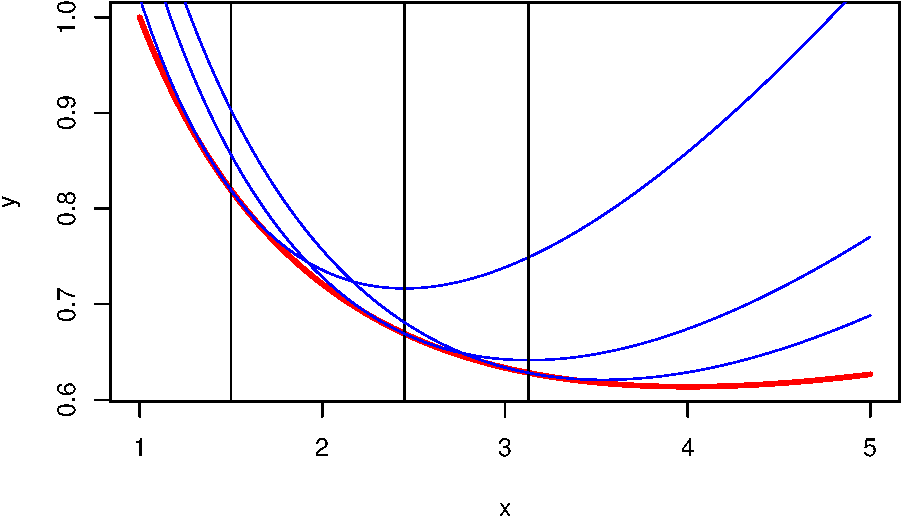
\includegraphics{smacofBS_files/figure-latex/majplot-1} \end{center}

\subsubsection{Majorizing Stress}\label{majorizing-stress}

\subsection{Second Phase: Update Transformation}\label{second-phase-update-transformation}

\subsubsection{Spline Basis Details}\label{spline-basis-details}

\emph{Splines} of degree \(d\) on a closed interval \([a,b]\) are piecewise polynomials of degree \(d\). The endpoints of the interval are the \emph{boundary knots}. In the interval there are a number of \emph{inner knots}. For smacof we suppose the inner knots are distinct. There is a polynomial piece between all consecutive
pairs of knots. Although the pieces can be parts of different polynomials
splines are required to have a certain degree of smoothness. In fact
at the interior knots a spline has \(d - 1\) continuous derivatives. A
spline of degree zero is a step function, stepping to a different level
at each knot. A spline of degree one is piecewise linear, where the
line segments are joined continuously at the inner knots. A spline of
degree two is piecewise quadratic and continuously differentiable at the
knots. And so on. There is no limit on the number of inner knots and
on the degree of the spline, although the number of interior knots
must be greater than or equal to the degree minus one. The flexibility
of the spline (as opposed to the rigidity of a polynomial on \([a,b]\)
of the same degree) comes from the number and placement of the interior knots, not so much from the degree of the spline.

\subsubsection{B-splines}\label{b-splines}

\subsubsection{Berstein PolynomiaLS}\label{berstein-polynomials}

\begin{longtable}[]{@{}ccccc@{}}
\caption{\label{tab:bsplinekable}B spline parameters}\tabularnewline
\toprule\noalign{}
degree & order & ninner & nknots & span \\
\midrule\noalign{}
\endfirsthead
\toprule\noalign{}
degree & order & ninner & nknots & span \\
\midrule\noalign{}
\endhead
\bottomrule\noalign{}
\endlastfoot
0 & 1 & 4 & 6 & 5 \\
1 & 2 & 4 & 8 & 6 \\
2 & 3 & 4 & 10 & 7 \\
3 & 4 & 4 & 12 & 8 \\
4 & 5 & 4 & 14 & 9 \\
\end{longtable}

\[
\sum_i B_{i,k}(x)=1
\]

M-splines

\[
M_{i,k}(x)=\frac{k+1}{t_{i+k+1}-t_i}B_{i,k}(X)
\] then \[
\int M_{i,k}(x)dx=1
\]

I-splines \[
I_{i,k+1}(z)=\int_{-\infty}^zM_{i,k}(x)dx
\]

When is a B-spline increasing ? \[
\mathcal{D}B_{i,k}(x)=
\] Thus if \[
\mathcal{D}\sum_{i=1}^{d+m}\alpha_iB_{i,k}(x)=
\]

It is sufficient that \(\alpha_i\leq\alpha_{i+1}\)

Integral, I-splines

\subsubsection{Ordinal MDS}\label{ordinal-mds}

\subsubsection{Interval and Ratio MDS}\label{interval-and-ratio-mds}

Additive constant

\subsubsection{Cyclic Coordinate Decent}\label{cyclic-coordinate-decent}

In the non-linear least squares (NNLS) problem the data are an
\(n\times p\) matrix \(X\), a vector \(y\) with \(n\) elements, and a positive
semi-definite diagonal matrix \(W\). We want to minimize \[
\sigma(\beta):=\frac12(X\beta-y)'W(X\beta-y)
\] over \(\beta\geq 0\). In data analysis and statistics the problem is
often solved by \emph{active set methods}, implemented in R for example by
NNLS (Mullen and van Stokkum (2023)) and FNNLS (Bro and De Jong (1997)). Active set
methods are finitely convergent dual methods. While iterating the
intermediate solutions are not feasible (i.e.~non-negative). In fact in
dual methods we reach feasibility and optimality at the same time. Also
the number of iterations, although theoretically finite, can be very
large.

In each smacof iteration we need an NNLS solution. Especially in the
early iterations the solution does not have to be very precise. Also the
solution from the previous NNLS problem will generally provide a very
good starting value for the next iteration (each NNLS problem has a ``hot
start''). And finally, we would like all internediate solutions to be
feasible. These considerations have lead us to using \emph{cyclic coordinate
descent} (CCD).

Suppose the current best feasible solution in CCD iteration \(k\) is
\(\beta^{(k)}\). The next CCD iteration changes each of the \(p\)
coordinates of \(\beta^{(k)}\) in turn, maintaining feasibility, while
keeping the other \(p-1\) coordinates fixed at their current values. Thus
within a CCD iteration \(k\) we create intermediate solutions
\(\beta^{(k,1)},\cdots,\beta^{(k,p)}\), where each of the intermediate
solutions \(\beta^{(k,r)}\) differs from the previous one
\(\beta^{(k,r-1)}\) in a single coordinate. For consistency we define
\(\beta^{(k,0)}:=\beta^{(k)}\). After the iteration is finished we set
\(\beta^{(k+1)}=\beta^{(k,p)}\).

Note that in smacof each iteration modifies the coordinates in the order
\(1,\cdots,p\), which explains why the method is called ``cyclic''. There
are variations of CCD in which the order within an iteration is random
or greedy (choose the coordinate which gives the largest improvement) or
zig-zag \(1,\cdots,p,p-1,\cdots,1\). We have not tried out these
alternatives in smacf, but we may in the future.

The effect of changing a single coordinate on the loss function is \[
\sigma(\beta+\epsilon e_j)=\sigma(\beta)+\epsilon\ g_j(\beta)+\frac12\epsilon^2s_{jj},
\] where \(e_j\) is the unit vector corresponding with the coordinate we
are changing, \(g(\beta):=\mathcal{D}\sigma(\beta)=X'Wr(\beta)\) is the
gradient at \(\beta\), and \(r(\beta):=X\beta-y\) is the residual. Also
\(S:=X'WX\). Note that if \(s_{jj}=0\) then also \(g_j(\beta)=0\) and thus
\(\sigma(\beta+\epsilon e_j)=\sigma(\beta)\). In each CCD cycle we simply
skip updating coordinate \(j\).

If \(s_{jj}>0\) then \(\sigma(\beta+\epsilon e_j)\) is a strictly convex
quadratic in \(\epsilon\), which we must minimize under the constraint
\(\beta_j+\epsilon\geq 0\) or \(\epsilon\geq-\beta_j\). Define
\(\hat\epsilon\) to be the solution of this constrained minimization
problem.

The quadratic \ldots{} has its minimum at \[
\tilde\epsilon=-\frac{g_j(\beta)}{s_{jj}}
\] If \(\beta+\tilde\epsilon\) is feasible then it is the update we are
looking for. Thus \(\hat\epsilon=\tilde\epsilon\). If
\(\beta+\tilde\epsilon<0\) then the contrained minimum is attained at the
boundary, i.e.~\(\hat\epsilon=-\beta_j\) and the updated \(\beta_j\) is
zero. Thus, in summary, \(\hat\epsilon=\max(\tilde\epsilon,-\beta_j)\).

One of the nice things about CCD is that \[
r(\hat\beta)=r(\beta)+\hat\epsilon x_j
\] \[
g(\hat\beta)=g(\beta)+\hat\epsilon s_j
\]

It follows that \(\hat\epsilon=0\) if and only if either \(\beta_j=0\) and
\(g_j(\beta)\geq 0\) or if \(g_j(beta)=0\) and \(beta_j>0\).

If \(g_j(\beta)<0\) then \(\tilde\epsilon>0\), and thus \(\hat\epsilon>0\) and
\(\sigma(\hat\beta)<\sigma(\beta)\). Thus we must have \(g_j(\beta)\geq 0\).

If \(\beta_j>0\) and \(g_j(\beta)\not=0\) then there is an \(\epsilon\) such
that \(\sigma(\beta+\epsilon e_j)<\sigma(\beta)\). Thus if \(\beta_j>0\) we
must have \(g_j(\beta)=0\).

In summary at the minimum of \(\sigma\) over \(\beta\geq 0\) we must have
\(\beta_j\geq 0\), \(g_j(\beta)\geq 0\), and \(\beta_jg_j(\beta)=0\) for all
\(j\) (\emph{complementary slackness}).

\[
\sigma(\beta+\epsilon e_j)=\sigma(\beta)+\epsilon\ g_j(\beta)+\frac12\epsilon^2s_{jj},
\] where \(S:=X'WX\).

Now suppose we minimize \(\sigma\) over \(\beta\geq 0\).

Our best solution so far is \(\beta^{(k)}\geq 0\). Minimize
\(\sigma(\beta^{(k)}+\epsilon e_1)\) over \(\epsilon\) on the condition that
\(\beta^{(k)}_1+\epsilon\geq 0\) or \(\epsilon\leq-\beta^{(k)}_1\). If
\(s_{11}=0\) then also \(g_1(\beta)=0\) and we set
\(\beta^{(k+1,1)}=\beta^{(k,1)}\). If \(s_{11}>0\) we compute \[
\tilde\epsilon=-g_1(\beta)/s_{11}
\] If \[
\beta^{(k)}_1+\tilde\epsilon\geq 0
\] then \[
\beta^{(k+1,1)}=\beta^{(k)}_1+\tilde\epsilon
\] If \[
\beta^{(k)}_1+\tilde\epsilon<0
\] we set \[
\beta^{(k+1,1)}=0.
\]

\section{Smacof Program}\label{smacof-program}

\subsubsection{Front-end}\label{front-end}

The front-end for both smacofBS and smacofRC is written in R. The
analysis is started in the user's working directory by the command
smacofBS(foo) or smacofRC(foo), where foo is a user-chosen name (without
quotes).

Two text files need to be present in the working directory. The first is
fooParameters.txt, where of course you substitute the user-chosen name
for foo. The second file is fooDelta.txt, which has the dissimilarities
below the diagonal in row-major order.

The parameter file has key-value format. Here is an example.

\begin{Shaded}
\begin{Highlighting}[]
\NormalTok{nobj   }\DecValTok{9}
\NormalTok{ndim   }\DecValTok{3}
\NormalTok{init   }\DecValTok{2}
\NormalTok{width   }\DecValTok{10}
\NormalTok{precision   }\DecValTok{6}
\NormalTok{haveweights   }\DecValTok{0}
\NormalTok{itmax  }\DecValTok{1000}
\NormalTok{epsi  }\DecValTok{10}
\NormalTok{verbose  }\DecValTok{1}
\NormalTok{ditmax  }\DecValTok{5}
\NormalTok{depsi  }\DecValTok{6}
\NormalTok{dverbose  }\DecValTok{0}
\NormalTok{kitmax  }\DecValTok{5}
\NormalTok{kepsi  }\DecValTok{6}
\NormalTok{kverbose  }\DecValTok{0}
\NormalTok{degree  }\DecValTok{3}
\NormalTok{haveknots  }\DecValTok{3}
\NormalTok{ninner  }\DecValTok{5}
\NormalTok{ordinal  }\DecValTok{1}
\NormalTok{anchor }\DecValTok{0}
\NormalTok{intercept  }\DecValTok{1}
\end{Highlighting}
\end{Shaded}

The parameter file is read first, using the R function read.table().
There is one key-value pair on each line, at the start of the line. The order of the lines does not matter. There can be additional comments or other text on
each line after the value field, as long as that text is space-separated
from the value field. Additional key-value lines with non-existing
parameters can be added at will.

Values of the parameters are put the local environment using R function
assign(), which means they are available to R throughout the smacof run.
Of course if we choose smacofRC the front-end needs to pass them to C
using C(), but they will be available again for the back-end.

The Delta file, and any subsequent optional input files, are read with
the R function scan(). Values are separated by spaces. They can be on a
single line, or laid out as a lower-triangular matrix, or whatever. The
function scan() only stops reading if it reaches the end-of-file.

We'll now discuss the parameters one by one. Note that all parameters
are integers. The first two are obvious: \emph{nobj} is the number of objects
and \emph{ndim} the number of dimensions. These two parameters have no
default or recommended values, because they deyermined by the data. All
other parameters in our example parameter file are set to reasonable
values in our example parameter file. But the whole idea is to
experiment with various combinations of parameter values, so
``reasonable'' is weaker than ``recommended'' and ``recommended'' is weaker
than ``default''.

The \emph{init} parameter can have values 1, 2, or 3. If \emph{init} equals 1 the
program reads an initial configuration from the file fooXinit.txt in the
working directory. The file has \emph{nobj} * \emph{ndim} numbers, the initial
configuration, in row-major format. If \emph{init} = 2 then the classical
Torgerson initial estimate will be computed. If \emph{init} = 3 a random
initial estimate will be used.

\emph{width} and \emph{precision} are parameters for the output of the values of
stress during iterations.

\emph{haveweights} is either zero or one. If zero there are no weights, which
is equivalent to all weights equal to one. If one then we will read a
file fooWeights.txt, which has the lower-diagonal \(\frac12 n(n-1)\)
weights in row-major order.

As explained in previous sections there are three iterative running in
smacof. There are two inner iterations: one for the configuration for
fixed disparities, and one for the disparities for fixed configuration.
The two inner iteration loops are nested in one outer iteration loop.
Each of the iterations has three parameters: one for the maximum number
of iterations, one for the stopping criterion, and one for the verbosity
of the iteration output. For the outer loop the parameters are \emph{itmax},
\emph{ieps}, and \emph{verbose}. For the inner configuration loop they are
\emph{kitmax}, \emph{keps}, and \emph{kverbose}. And the inner transformation loop they
are \emph{ditmax}, \emph{deps}, and \emph{dverbose}. If the verbose parameter is one,
then each iteration prints out the stress before and the stress after
update. If verbose is zero, nothing is printed. The stopping parameters
check if the change in stress in an iteration is less than epsilon,
where epsilon is 10\^{}-ieps, 10\^{}-keps, or 10\^{}-deps.

The final five parameters are used to define the nature of the spline
space for the transformations. \emph{degree} is the degree of the piecewise
polynomials. The \emph{haveknots} parameter can be 0, 1, 2, or 3. If it is
zero, there are no inner knots and we use the Bernstein polynomial
basis. If \emph{haveknots} is one, the inner knots are read in from
fooKnots.txt in the usual way. If \emph{haveknots} is two the knots are
equally spaced between zero and one, and if it is three the knots are
equally spaced on the precentile scale (so that the number of data
points between knots is approximately the same). The \emph{ninner} parameter
determines the number of knots in the case that \emph{haveknots} is either
two or three. If \emph{haveknots} is zero, then \emph{ninner} should be zero, if
\emph{haveknots} is one it should be equal to the number of knots in
fooKnots.txt.

The three final spline parameters are \emph{ordinal}, \emph{anchor}, and \emph{intercept}. If \emph{ordinal} is one the fitted spline is constrained to be monotone. If \emph{intercept} is zero then the first spline coefficient is constrained to be zero (which
means the first column is deleted from the basis). This means that the spline
is constrained to be zero at the lower boundary knot. If \emph{intercept} is one
there is no such constraint, and the spline can be anything at the lower boundary
(subject to monotonicity of \emph{ordinal} is one). If \emph{anchor} is one then the
boundary knots are set to zero and the maximum dissimilarity, if \emph{anchor} is
zero the boundary knots are the minimum and maximum dissimilarity. Thus if \emph{intercept} is zero and \emph{anchor} is one the spline goes through the origin.

The computations in the frontend are straightforward. We first transform
the dissimilarities linearly so that the smallest becomes zero and the
largest becomes one. This is not strictly necessary but it makes the
spline computations slightly easier.

Initial Estimates for \(X\) Spline Basis

\subsubsection{Engine}\label{engine}

ALS First Phase Second Phase

\subsubsection{Back-end}\label{back-end}

The back-end consists of a number of R functions that have the list
returned by smacofBS or smacofRC as an argument. They can be used to
make plots, compute derivatives, convert matrices to an easily
printable format, do sensitivity analysis, and so on. The philosophy
is that in the backend the main computing is finished and we
just create different representations of the results.

\paragraph{Plotting}\label{plotting}

There are two main plot functions in the backend: smacofShepardPlot()
and smacofConfigurationPlot(). A smacofShepardPlot has the
dissimilarities (un-normalized) on the horizontal axes and
it has the distances and the disparities on the vertical axis.
It draws the spline, and shows where the fitted disparities are
on the spline. It also plots the (delta, dist) pairs as points,
to show how far they deviate from the spline. Optionally
smacofShepardPlot() can draw vertical lines at the inner knots
(argument knotlines = TRUE), and optionally it can connect
the (delta, dhat) points on the spline to the (delta, dist)
points with lines (argument fitlines = TRUE).

It must be emphasized that smacofShepardPlot() draws the spline
over the whole interval, which is either (deltamin, deltamax)
if anchor = 0 and (0, deltamax) if anchor = 1. It does
this by recomputing the spline at a large number of
uniformly spaced points in the interval, where the
number of points is given by the smacofShepardPlot()
parameter resolution. Thus we do not use only the
data points (delta,dhat) and then let the R plot function
interpolate linearly. That can be misleading. It is
especially misleading if degree is zero (step function)
or if there are consecutive inner knots with no data values
between the knots. Degree zero is handled by the special
purpose step function plotting routine smacofPlotStepFunction(),
which makes sure the spline is drawn as a horizontal segment
from one knot to the next knot. In addition smacofShepardPlot()
can set some base R plot parameters such as col, cex, lwd, and pch
(see the R documentation).

The smacofConfigurationPlot() function is much simpler than
smacofShepardPlot(). It sets pch, col, and cex. It uses
the smacofBS/RC labels parameter to decide how to label
the points in the configuration. If labels = 1 it reads
a character vector of labels from fooLabels.txt, where
foo is of course the name of the run. If labels = 2
the points are numbered, if labels = 3 plotting uses
the pch symbol for all points. If the dimension \(p\)
is larger than two, smacofConfigurationPlot() uses
the parameters dim1 and dim2 to select the dimensions
to plot.

\paragraph{Writing}\label{writing}

\paragraph{Checking}\label{checking}

\paragraph{Derivatives}\label{derivatives}

\paragraph{Sensitivity}\label{sensitivity}

Perturbation regions

Parametric Bootstrap

Jacknife

\section{Examples}\label{examples}

\subsection{ekman}\label{ekman}

The Ekman (1954) color circle similarities have been used in many, if not most, multidimensional scaling textbooks and review articles. See, for example,
Borg and Groenen (2005), p 63-68. Its popularity is due, no doubt,
to its astonishing good two-dimensional fit and its easy interpretability.

In brief, Ekman used what he called the \emph{Method of similarity analysis}. The stimuli
were fourteen color filters, transmitting light of wave lengths 434 \(m\mu\) mp to 674 \(m\mu\). The subjects were 31 students with normal color vision. They judged
the similarity between all 91 pairs of colors on a five-point rating scale
with categories 0-4. The similarity judgments were then averaged over students
and the average was divided by four to create similarties \(s_{ij}\) between zero
and one. For MDS purposes we set \(\delta_{ij}=1-s_{ij}\).

We start with a metric analysis in two dimensions. In all analyses in this section of the manual we start with the Torgerson initial configuration, and we iterate until the change in stress from one outer iteration to the next is less than or equal to 1e-10.

After 32 iterations we find a minimum stress of 0.5278528. The Shepardplot in the left panel of figure \ref{fig:ekmanmetric} shows a reasonably
good fit, but strongly suggests making a non-linear transformation to improve the fit.

It is known that if we use \(\delta_{ij}=(1-s_{ij})^3\) then the two-dimensional solution computed by smacof is the
global minimum of stress for all dimensions \(p\geq 2\) (De Leeuw (2014), De Leeuw (2019)). So we repeated the metric analysis using the cubic transformation.
After 17 iterations we find stress 0.2426954 and the Shepardplot in the right panel of figure \ref{fig:ekmanmetric}. A better fit, and
the deviations from linearity are what one expects from least squares: overestimation
of the smaller dissimilarities and underestimation of the larger ones. Nevertheless,
the configurations for the two solutions in figure \ref{fig:ekmanmetricconf} are remarkably similar, showing once again that configurations tend to be more stable than Shepardplots.

\begin{greybox}

\begin{center}
\textbf{INSERT FIGURE \ref{fig:ekmanmetric} ABOUT HERE}

\end{center}

\end{greybox}

\begin{greybox}

\begin{center}
\textbf{INSERT FIGURE \ref{fig:ekmanmetricconf} ABOUT HERE}

\end{center}

\end{greybox}

We present four additional non-metric analyses, using the seven-digit coding
illustrated in table \ref{tab:ekmankable}. The stress values in the table cannot be compared directly with those of the metric solutions, because in the non-metric analysis the dissimilarities are normalized and thus the stress scales are different. We can compare within the table, however, and compare all Shepard plots.

\begin{greybox}

\begin{center}
\textbf{INSERT TABLE \ref{tab:ekmankable} ABOUT HERE}

\end{center}

\end{greybox}

\begin{greybox}

\begin{center}
\textbf{INSERT FIGURE \ref{fig:ekmancubic} ABOUT HERE}

\end{center}

\end{greybox}

\begin{greybox}

\begin{center}
\textbf{INSERT FIGURE \ref{fig:ekmanordinal} ABOUT HERE}

\end{center}

\end{greybox}

\subsection{gruijter}\label{gruijter}

The ekman examples had a really good fit. We use the data from De Gruijter (1967)
for an example with a rather bad fit in two dimensions.
Dissimilarity judgments between nine Dutch political parties were
collected in 1966 by the complete method of triads. Results were
averaged over 100 students. Averaging over a heterogeneous population
will cause regression to the mean, and thus dissimilarities will tend
to be more equal than they should be on the basis of the individual
results. This means there should be a substantial difference in fit between
the ``ratio'' and the ``interval'' options
(i.e.~between the interval parameter equal to one or zero).

\subsection{morse}\label{morse}

\section{Tables}\label{tables}

\begin{longtable}[]{@{}
  >{\centering\arraybackslash}p{(\columnwidth - 16\tabcolsep) * \real{0.1013}}
  >{\centering\arraybackslash}p{(\columnwidth - 16\tabcolsep) * \real{0.1013}}
  >{\centering\arraybackslash}p{(\columnwidth - 16\tabcolsep) * \real{0.1392}}
  >{\centering\arraybackslash}p{(\columnwidth - 16\tabcolsep) * \real{0.1139}}
  >{\centering\arraybackslash}p{(\columnwidth - 16\tabcolsep) * \real{0.1392}}
  >{\centering\arraybackslash}p{(\columnwidth - 16\tabcolsep) * \real{0.1013}}
  >{\centering\arraybackslash}p{(\columnwidth - 16\tabcolsep) * \real{0.0759}}
  >{\centering\arraybackslash}p{(\columnwidth - 16\tabcolsep) * \real{0.1519}}
  >{\centering\arraybackslash}p{(\columnwidth - 16\tabcolsep) * \real{0.0759}}@{}}
\caption{\label{tab:ekmankable}Analyses of the ekman example}\tabularnewline
\toprule\noalign{}
\begin{minipage}[b]{\linewidth}\centering
ninner
\end{minipage} & \begin{minipage}[b]{\linewidth}\centering
degree
\end{minipage} & \begin{minipage}[b]{\linewidth}\centering
haveknots
\end{minipage} & \begin{minipage}[b]{\linewidth}\centering
ordinal
\end{minipage} & \begin{minipage}[b]{\linewidth}\centering
intercept
\end{minipage} & \begin{minipage}[b]{\linewidth}\centering
anchor
\end{minipage} & \begin{minipage}[b]{\linewidth}\centering
ndim
\end{minipage} & \begin{minipage}[b]{\linewidth}\centering
stress
\end{minipage} & \begin{minipage}[b]{\linewidth}\centering
itel
\end{minipage} \\
\midrule\noalign{}
\endfirsthead
\toprule\noalign{}
\begin{minipage}[b]{\linewidth}\centering
ninner
\end{minipage} & \begin{minipage}[b]{\linewidth}\centering
degree
\end{minipage} & \begin{minipage}[b]{\linewidth}\centering
haveknots
\end{minipage} & \begin{minipage}[b]{\linewidth}\centering
ordinal
\end{minipage} & \begin{minipage}[b]{\linewidth}\centering
intercept
\end{minipage} & \begin{minipage}[b]{\linewidth}\centering
anchor
\end{minipage} & \begin{minipage}[b]{\linewidth}\centering
ndim
\end{minipage} & \begin{minipage}[b]{\linewidth}\centering
stress
\end{minipage} & \begin{minipage}[b]{\linewidth}\centering
itel
\end{minipage} \\
\midrule\noalign{}
\endhead
\bottomrule\noalign{}
\endlastfoot
0 & 3 & 0 & 1 & 0 & 1 & 2 & 0.08686091 & 118 \\
5 & 3 & 3 & 1 & 0 & 1 & 2 & 0.07869019 & 2944 \\
50 & 0 & 3 & 1 & 0 & 1 & 2 & 0.04675950 & 1296 \\
50 & 0 & 2 & 1 & 0 & 1 & 2 & 0.05895210 & 885 \\
\end{longtable}

\begin{center}\rule{0.5\linewidth}{0.5pt}\end{center}

\begin{longtable}[]{@{}
  >{\centering\arraybackslash}p{(\columnwidth - 16\tabcolsep) * \real{0.1013}}
  >{\centering\arraybackslash}p{(\columnwidth - 16\tabcolsep) * \real{0.1013}}
  >{\centering\arraybackslash}p{(\columnwidth - 16\tabcolsep) * \real{0.1392}}
  >{\centering\arraybackslash}p{(\columnwidth - 16\tabcolsep) * \real{0.1139}}
  >{\centering\arraybackslash}p{(\columnwidth - 16\tabcolsep) * \real{0.1392}}
  >{\centering\arraybackslash}p{(\columnwidth - 16\tabcolsep) * \real{0.1013}}
  >{\centering\arraybackslash}p{(\columnwidth - 16\tabcolsep) * \real{0.0759}}
  >{\centering\arraybackslash}p{(\columnwidth - 16\tabcolsep) * \real{0.1519}}
  >{\centering\arraybackslash}p{(\columnwidth - 16\tabcolsep) * \real{0.0759}}@{}}
\caption{\label{tab:gruijterkable}Analyses of the gruijter example}\tabularnewline
\toprule\noalign{}
\begin{minipage}[b]{\linewidth}\centering
ninner
\end{minipage} & \begin{minipage}[b]{\linewidth}\centering
degree
\end{minipage} & \begin{minipage}[b]{\linewidth}\centering
haveknots
\end{minipage} & \begin{minipage}[b]{\linewidth}\centering
ordinal
\end{minipage} & \begin{minipage}[b]{\linewidth}\centering
intercept
\end{minipage} & \begin{minipage}[b]{\linewidth}\centering
anchor
\end{minipage} & \begin{minipage}[b]{\linewidth}\centering
ndim
\end{minipage} & \begin{minipage}[b]{\linewidth}\centering
stress
\end{minipage} & \begin{minipage}[b]{\linewidth}\centering
itel
\end{minipage} \\
\midrule\noalign{}
\endfirsthead
\toprule\noalign{}
\begin{minipage}[b]{\linewidth}\centering
ninner
\end{minipage} & \begin{minipage}[b]{\linewidth}\centering
degree
\end{minipage} & \begin{minipage}[b]{\linewidth}\centering
haveknots
\end{minipage} & \begin{minipage}[b]{\linewidth}\centering
ordinal
\end{minipage} & \begin{minipage}[b]{\linewidth}\centering
intercept
\end{minipage} & \begin{minipage}[b]{\linewidth}\centering
anchor
\end{minipage} & \begin{minipage}[b]{\linewidth}\centering
ndim
\end{minipage} & \begin{minipage}[b]{\linewidth}\centering
stress
\end{minipage} & \begin{minipage}[b]{\linewidth}\centering
itel
\end{minipage} \\
\midrule\noalign{}
\endhead
\bottomrule\noalign{}
\endlastfoot
0 & 1 & 0 & 0 & 0 & 1 & 3 & 0.23524290 & 42 \\
0 & 1 & 0 & 0 & 1 & 0 & 3 & 0.06099819 & 43 \\
0 & 3 & 0 & 1 & 0 & 1 & 2 & 0.34953364 & 106 \\
0 & 3 & 0 & 1 & 0 & 1 & 3 & 0.07248619 & 115 \\
5 & 3 & 3 & 1 & 0 & 1 & 2 & 0.34082527 & 667 \\
5 & 3 & 3 & 1 & 0 & 1 & 3 & 0.04823789 & 614 \\
\end{longtable}

\begin{center}\rule{0.5\linewidth}{0.5pt}\end{center}

\section{Figures}\label{figures}

\begin{figure}

{\centering 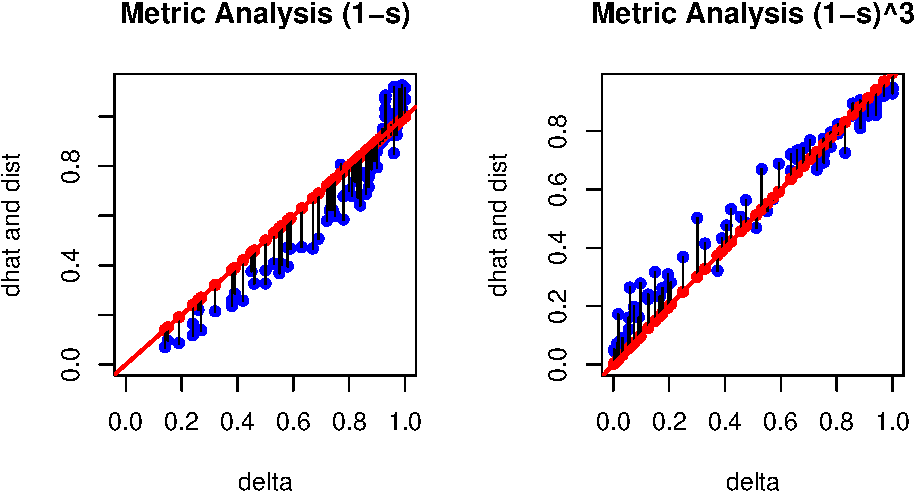
\includegraphics{smacofBS_files/figure-latex/ekmanmetric-1} 

}

\caption{ekman example, metric}\label{fig:ekmanmetric}
\end{figure}

\begin{figure}

{\centering 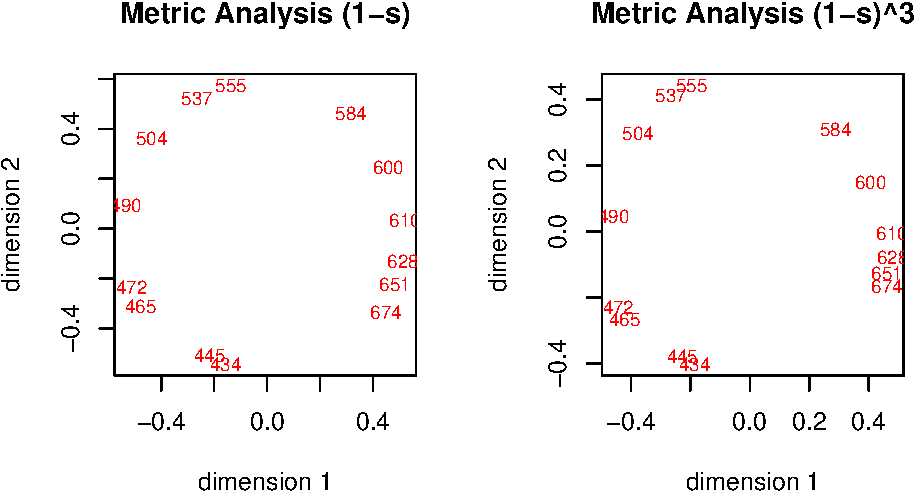
\includegraphics{smacofBS_files/figure-latex/ekmanmetricconf-1} 

}

\caption{ekman example, metric}\label{fig:ekmanmetricconf}
\end{figure}

\begin{figure}

{\centering 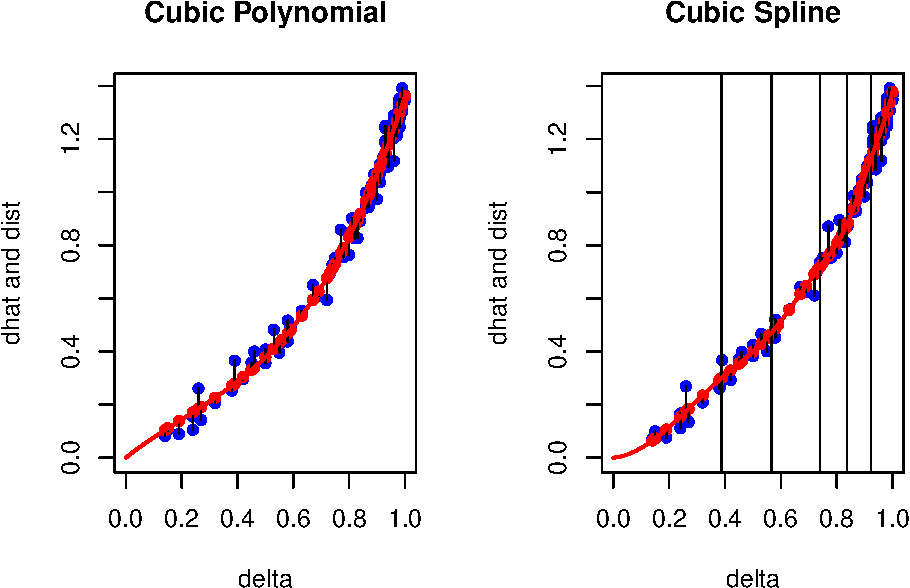
\includegraphics{smacofBS_files/figure-latex/ekmancubic-1} 

}

\caption{ekman example, cubic analysis}\label{fig:ekmancubic}
\end{figure}

\begin{figure}

{\centering 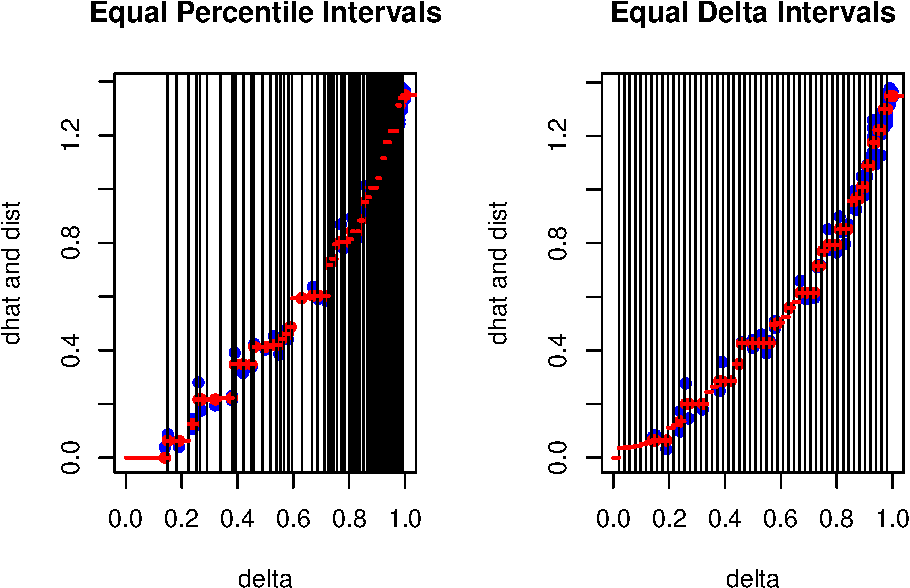
\includegraphics{smacofBS_files/figure-latex/ekmanordinal-1} 

}

\caption{ekman example, pseudo-nonmetric analysis}\label{fig:ekmanordinal}
\end{figure}

\begin{figure}

{\centering 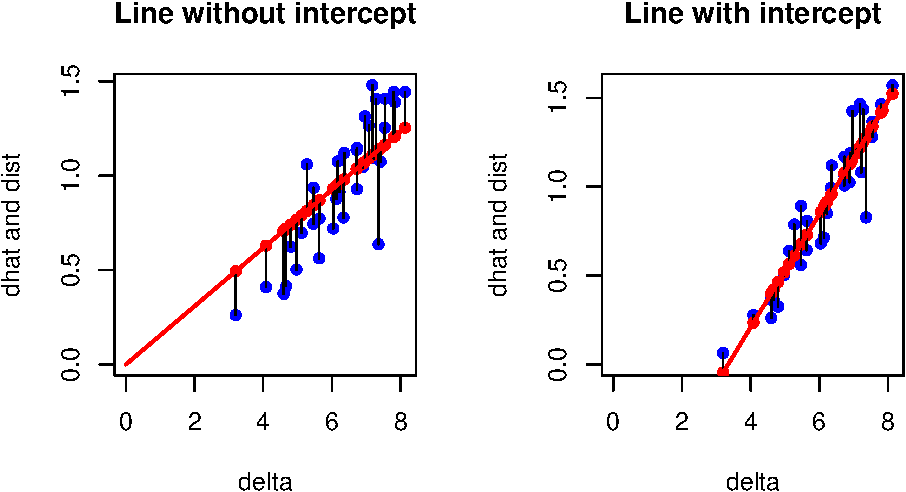
\includegraphics{smacofBS_files/figure-latex/gruijterlinear-1} 

}

\caption{gruijter example, linear analysis}\label{fig:gruijterlinear}
\end{figure}

\begin{figure}

{\centering 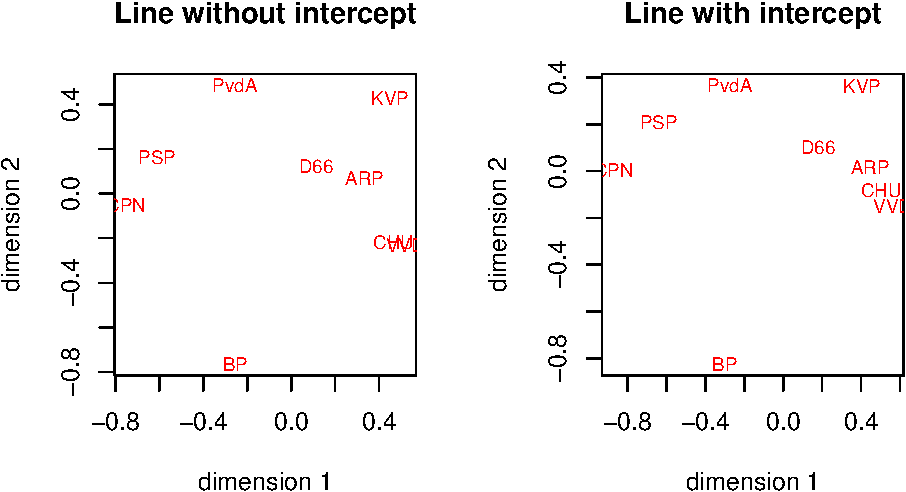
\includegraphics{smacofBS_files/figure-latex/gruijterlinearconf-1} 

}

\caption{gruijter example, linear analysis}\label{fig:gruijterlinearconf}
\end{figure}

\begin{figure}

{\centering 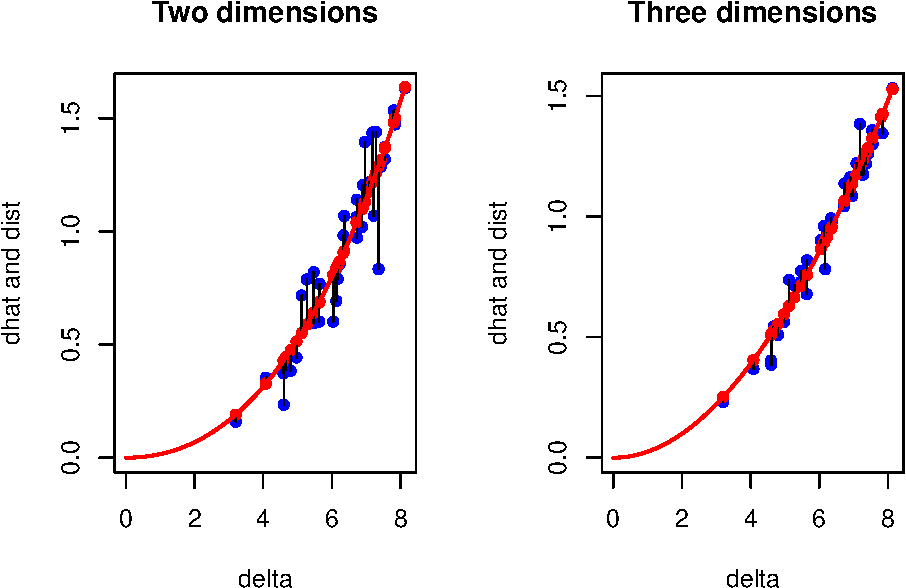
\includegraphics{smacofBS_files/figure-latex/gruijtercubic-1} 

}

\caption{gruijter example, cubic polynomial}\label{fig:gruijtercubic}
\end{figure}

\begin{figure}

{\centering 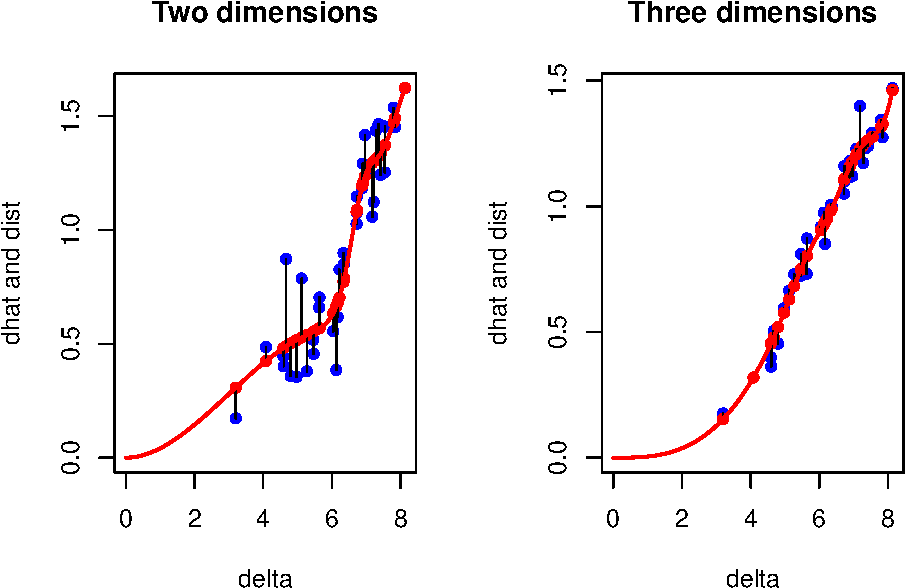
\includegraphics{smacofBS_files/figure-latex/gruijtersplines-1} 

}

\caption{gruijter example, cubic spline analysis}\label{fig:gruijtersplines}
\end{figure}

\section*{References}\label{references}
\addcontentsline{toc}{section}{References}

\phantomsection\label{refs}
\begin{CSLReferences}{1}{0}
\bibitem[\citeproctext]{ref-boehning_lindsay_88}
Böhning, D., and B. G. Lindsay. 1988. {``{Monotonicity of Quadratic-approximation Algorithms}.''} \emph{Annals of the Institute of Statistical Mathematics} 40 (4): 641--63.

\bibitem[\citeproctext]{ref-borg_groenen_05}
Borg, I., and P. J. F. Groenen. 2005. \emph{Modern Multidimensional Scaling}. Second Edition. Springer.

\bibitem[\citeproctext]{ref-bro_dejong_97}
Bro, R., and S. De Jong. 1997. {``A Fast Non-Negatively-Constrained Least Squares Algorithm.''} \emph{Journal of Chemometrics} 11: 393--401.

\bibitem[\citeproctext]{ref-degruijter_67}
De Gruijter, D. N. M. 1967. {``{The Cognitive Structure of Dutch Political Parties in 1966}.''} Report E019-67. Psychological Institute, University of Leiden.

\bibitem[\citeproctext]{ref-deleeuw_C_77}
De Leeuw, J. 1977. {``Applications of Convex Analysis to Multidimensional Scaling.''} In \emph{Recent Developments in Statistics}, edited by J. R. Barra, F. Brodeau, G. Romier, and B. Van Cutsem, 133--45. Amsterdam, The Netherlands: North Holland Publishing Company.

\bibitem[\citeproctext]{ref-deleeuw_C_94c}
---------. 1994. {``{Block Relaxation Algorithms in Statistics}.''} In \emph{Information Systems and Data Analysis}, edited by H. H. Bock, W. Lenski, and M. M. Richter, 308--24. Berlin: Springer Verlag. \url{https://jansweb.netlify.app/publication/deleeuw-c-94-c/deleeuw-c-94-c.pdf}.

\bibitem[\citeproctext]{ref-deleeuw_U_14b}
---------. 2014. {``{Bounding, and Sometimes Finding, the Global Minimum in Multidimensional Scaling}.''} UCLA Department of Statistics. \url{https://jansweb.netlify.app/publication/deleeuw-u-14-b/deleeuw-u-14-b.pdf}.

\bibitem[\citeproctext]{ref-deleeuw_E_19e}
---------. 2019. {``{Global Minima by Penalized Full-dimensional Scaling}.''} 2019. \url{https://jansweb.netlify.app/publication/deleeuw-e-19-e/deleeuw-e-19-e.pdf}.

\bibitem[\citeproctext]{ref-dempster_laird_rubin_77}
Dempster, A. P., N. M. Laird, and D. B. Rubin. 1977. {``{Maximum Likelihood for Incomplete Data via the EM Algorithm}.''} \emph{Journal of the Royal Statistical Society} B39: 1--38.

\bibitem[\citeproctext]{ref-ekman_54}
Ekman, G. 1954. {``{Dimensions of Color Vision}.''} \emph{Journal of Psychology} 38: 467--74.

\bibitem[\citeproctext]{ref-lange_16}
Lange, K. 2016. \emph{MM Optimization Algorithms}. SIAM.

\bibitem[\citeproctext]{ref-lethi_tao_18}
Le Thi, H. A., and P. D. Tao. 2018. {``{DC Programming and DCA: Thirty Years of Developments}.''} \emph{Mathematical Programming, Series B}.

\bibitem[\citeproctext]{ref-mullen_vanstokkum_23}
Mullen, K. M., and I. H. M. van Stokkum. 2023. \emph{{nnls: The Lawson-Hanson algorithm for non-negative least squares (NNLS)}}. \url{\%7Bhttps://CRAN.R-project.org/package=nnls\%7D}.

\bibitem[\citeproctext]{ref-nikolova_ng_05}
Niikolova, M., and M. Ng. 2005. {``Analysis of Half-Quadratic Minimization Methods for Signal and Image Recovery.''} \emph{SIAM Journal Scientific Computing} 27 (3): 937--66.

\bibitem[\citeproctext]{ref-vosz_eckhardt_80}
Vosz, H., and U. Eckhardt. 1980. {``{Linear Convergence of Generalized {W}eiszfeld's Method}.''} \emph{Computing} 25: 243--51.

\bibitem[\citeproctext]{ref-yuille_rangarajan_03}
Yuille, A. L., and A. Rangarajan. 2003. {``{The Concave-Convex Procedure}.''} \emph{Neural Computation} 15: 915--36.

\bibitem[\citeproctext]{ref-zangwill_69a}
Zangwill, W. I. 1969. \emph{{Nonlinear Programming: a Unified Approach}}. Englewood-Cliffs, N.J.: Prentice-Hall.

\end{CSLReferences}

\end{document}
